\documentclass[lecture.tex]{subfiles}

\begin{document}

\exercice{}
%\video{https://youtu.be/blablabla}
\enonce{rdm-0009}{Poutre en appuie chargée}


\begin{center}
  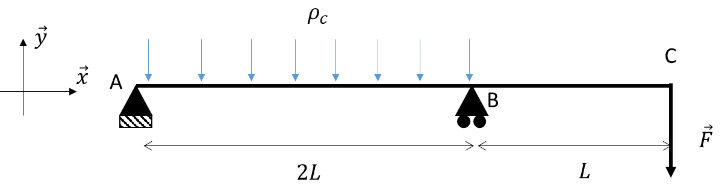
\includegraphics[scale=0.5]{exo-poutre-en-appuie-chargee.png}
\end{center}

\begin{enumerate}
  \item Déterminer le degré d’hyperstatisme de la poutre.
  \item Trouver les inconnus de liaison de la structure (les efforts et les moments résultants des deux liaisons).
  \item De combien de coupe a-on-t besoin pour étudier les efforts internes
  \item Etudier les efforts internes de la poutre
\end{enumerate}

\finenonce{rdm-0009}
\finexercice

\end{document}
